% Source: source_md/intelligence_part2_combined_ja.md
\section{社会的ブロックチェーン — $\Phi_{\text{net}}$ としての分散 $L_E$}

\noindent\textbf{記述の射程。} 社会的ブロックチェーンの非技術的・モデル内の命名を維持する。ネットワーク運用と歴史的系列は提案的解釈であり、実装済み合意protocolや進歩法則ではない。Gitと社会のcost対照は共通実測尺度のない仮説である。正統性が社会的受容に依存することから原理的非計算可能性は確立されない。個体創造と社会安定化の対照は役割仮説であり、創造の排他法則ではない。記録・正統性・創造・共有停止の独立基準は未解決である。

本章の要約と歴史図を含め、社会的logと分散停止は宣言network scopeで扱い、個体のLR・LEへ自動移送しない。共有記録は生成履歴の全体ではなく、networkでの保持は各個体の役割やownnessの認証ではない。第5節のsupport・role・証拠の区別をarchitecture比較に適用し、同期機構が成立したとはしない。



\S{}6〜\S{}8 で、$L_E$ が環境直接相互干渉(アニミズム)、中心化(神)、世代横断的維持(宗教)という形態を取ることを見た。本章は、停止構造を単一権威に依存させずに維持する形態——分散的社会停止——を扱う。これを「社会的ブロックチェーン」と呼ぶ。

まず用語について明確にしておく。本章の「ブロックチェーン」は、暗号通貨や分散台帳の特定の技術を指すものではない。それは、単一権威なしに停止と更新を両立させる構造の特徴を捉えるための、構造的アナロジーである。本論文が借りるのは技術の実装ではなく、その構造的特徴——分散したノードが、中央権威なしに、暫定的合意を形成し、それを更新可能に保つ——だけである。

\bigskip


\subsection{社会的ブロックチェーンの構造的特徴}


社会的ブロックチェーンの中心的特徴は、単一権威なしでの停止と更新の共存である。

\S{}7〜\S{}8 で見た中心化された停止構造(神・宗教)は、停止の曖昧性を低減する代わりに、中心化された参照点の硬直化リスクを負った(\S{}8.5、\S{}8.8)。社会的ブロックチェーンは、このトレードオフに対する別の構造的応答である。それは停止を単一の参照点に集約せず、分散したノード間で維持する。同時に、その停止を固定せず、更新可能に保つ。

停止と更新を分散構造に関係づけることを、社会的ブロックチェーンという語で提案する。個々の判断の暫定性とネットワークの更新を比較するが、その両立が達成されていると確認したものではない。

これは \S{}5.8 の改訂可能性を社会的スケールで読む役割類比であり、実装済みの橋渡しではない。

\bigskip


\subsection{構成要素}


社会的ブロックチェーンの構造を、その構成要素によって記述する。これらは技術的ブロックチェーンの用語からの構造的借用である。

\begin{itemize}
\item \textbf{個体ノード}: 判断を生成する単位。各個体は自らの $L_F$ で推論し、$L_E$ で暫定的停止を生成する。
\item \textbf{ログ}: 永続的な記録。個体ノードの判断とその根拠が記録され、参照可能に保たれる(\S{}5.2 の $L_R$ の社会的拡張)。
\item \textbf{ブロック}: 暫定的に採用された判断。複数のノードによって受容され、当面の停止点として機能する判断の単位。
\item \textbf{フォーク}: 判断の分岐。同一の問題に対して異なる停止が並立する状態。\S{}3.7 の分岐構造の社会的現れ。
\item \textbf{マージ/破棄}: 分岐した判断の統合または放棄。フォークが解消され、停止が再編される過程。
\end{itemize}


ノード、ログ、ブロック、フォーク、マージ/破棄を、判断・記録・暫定採用・分岐・再編の役割として比較する。単一権威なしにこの循環が必ず持続するという機構の検証ではない。

\bigskip


\subsection{バージョン管理システムとの対比}


社会的ブロックチェーンの性格を明確にするため、技術的なバージョン管理システム(Git のような)と対比する。両者はともに分散・分岐・統合の構造を持つが、その動力学的目的が異なる。

技術的バージョン管理の分岐・マージ・ロールバックを、探索の支援という観点から比較する。ただし、それらのコストや目的は利用条件に依存し、一律の最適化法則としては扱わない。

社会的ブロックチェーンの比喩では、分岐・合意・撤回に伴う負担を考える。これらが技術的システムより常に高コストであることや、社会が事後安定化だけを最大化することは確立していない。

この対比は次のように整理される:

\begin{longtable}{@{}p{0.30\linewidth}p{0.30\linewidth}p{0.30\linewidth}@{}}
\toprule
 & 技術的バージョン管理 & 社会的ブロックチェーン \\
\midrule
\endfirsthead
\toprule
 & 技術的バージョン管理 & 社会的ブロックチェーン \\
\midrule
\endhead
動力学的目的 & 創造的探索の最大化 & 事後安定化の最大化 \\
分岐コスト & 低い & 高い \\
マージ速度 & 速い & 遅い \\
ロールバック & 容易 & 困難 \\
失敗の重み & 小さい & 大きい \\
\bottomrule
\end{longtable}


両者のコストの対比は定性的な類比であり、対称的な反転則ではない。探索と安定化という役割の割当から、コストの大小を導くことはしない。

\bigskip


\subsection{一貫性ではなく正統性}


技術的ブロックチェーンと社会的ブロックチェーンの最も深い差異は、何を問題とするかにある。

技術的ブロックチェーンは、一貫性 (consistency) の問題を扱う。分散したノードが、矛盾のない単一の状態に合意できるか。これは計算的に定式化可能な問題であり、合意アルゴリズムによって解決される。

社会的ブロックチェーンは、正統性 (legitimacy) の問題を扱う。分散したノードが受容する停止が、正統なものとして成立するか。この社会的読解から原理的な非計算可能性は確立されない。

正統性を時間・責任・歴史・分散的受容に関係するものとして仮説化する。誰がいつ受容し、その受容がどれだけ持続し、誰が責任を負ったかという読解は、アルゴリズムによる扱いの原理的不可能性を証明しない。

技術的ブロックチェーンの一貫性と社会的正統性は異なる負担を持つ。後者について、$\Phi_{\text{net}}$ における $L_E$ の相互干渉という歴史的読解を提案するが、非計算可能性の形式的結果ではない。

社会的停止構造を改訂可能な歴史的過程として読む仮説は保持する。ただし計算可能性と固定化、\S{}8.5 の硬直化リスクとの必然的関係は未確立であり、非計算可能性を改訂可能性の説明に使わない。

\bigskip


\subsection{個体創造と社会的安定化の役割仮説}


社会的ブロックチェーンについて、個体の創造と社会的安定化を対照する役割仮説を述べる。社会的創造を排除する法則ではない。

社会的ブロックチェーンは事後安定化のために動いている(\S{}9.3)。その機能は、生成された判断を受容し、安定化し、改訂可能に保つことである。これは創造の機能ではない。ここでは社会を判断の安定化という役割から読むが、判断の創造を一般に否定しない。

個体ノードの創造を $L_F$ の動きや \S{}3.8 の不安定領域、準閉包 $\Omega_\theta$ の境界と関連づける仮説である。新しい概念や仮説の生成がこの接続で説明されたことや、創造が個体だけに起こることは確立していない。

ここに、知性の三層動力学における役割分担が現れる。個体ノードは創造する($L_F$ の境界探索)。社会は安定化する($\Phi_{\text{net}}$ の事後受容)。両者は異なる動力学的機能を担い、一方が他方を代替することはできない。この役割対照から社会の創造不能や個体の単独安定化不能を一般化しない(\S{}3、\S{}5)。

この役割分担を \S{}11 の不安定領域と比較する。個体の創造と社会の事後安定化という対応は構造的仮説であり、この分業が知性の持続に必ず必要であるとはしない。

\bigskip


\subsection{三層動力学における位置 — $\Phi_{\text{net}}$ そのものの一形態}


社会的ブロックチェーンを三層動力学の語彙で総括する。

社会的ブロックチェーンは、$\Phi_{\text{net}}$ そのものの一形態である。より正確には、$\Phi_{\text{net}}$——個体間 $L_E$ の相互干渉ネットワーク——を、明示的な分散構造として運用する形態である。

\S{}6〜\S{}8 の形態と対比すると、その位置が明確になる。アニミズムは $L_E$ を環境に分散させた。神は $L_E$ を中心化した。宗教は中心化された $L_E$ を世代横断的に維持した。社会的ブロックチェーンは、$L_E$ ネットワークそのものを、中心化せずに、明示的な分散構造として運用する。

\begin{figure}[H]
\centering
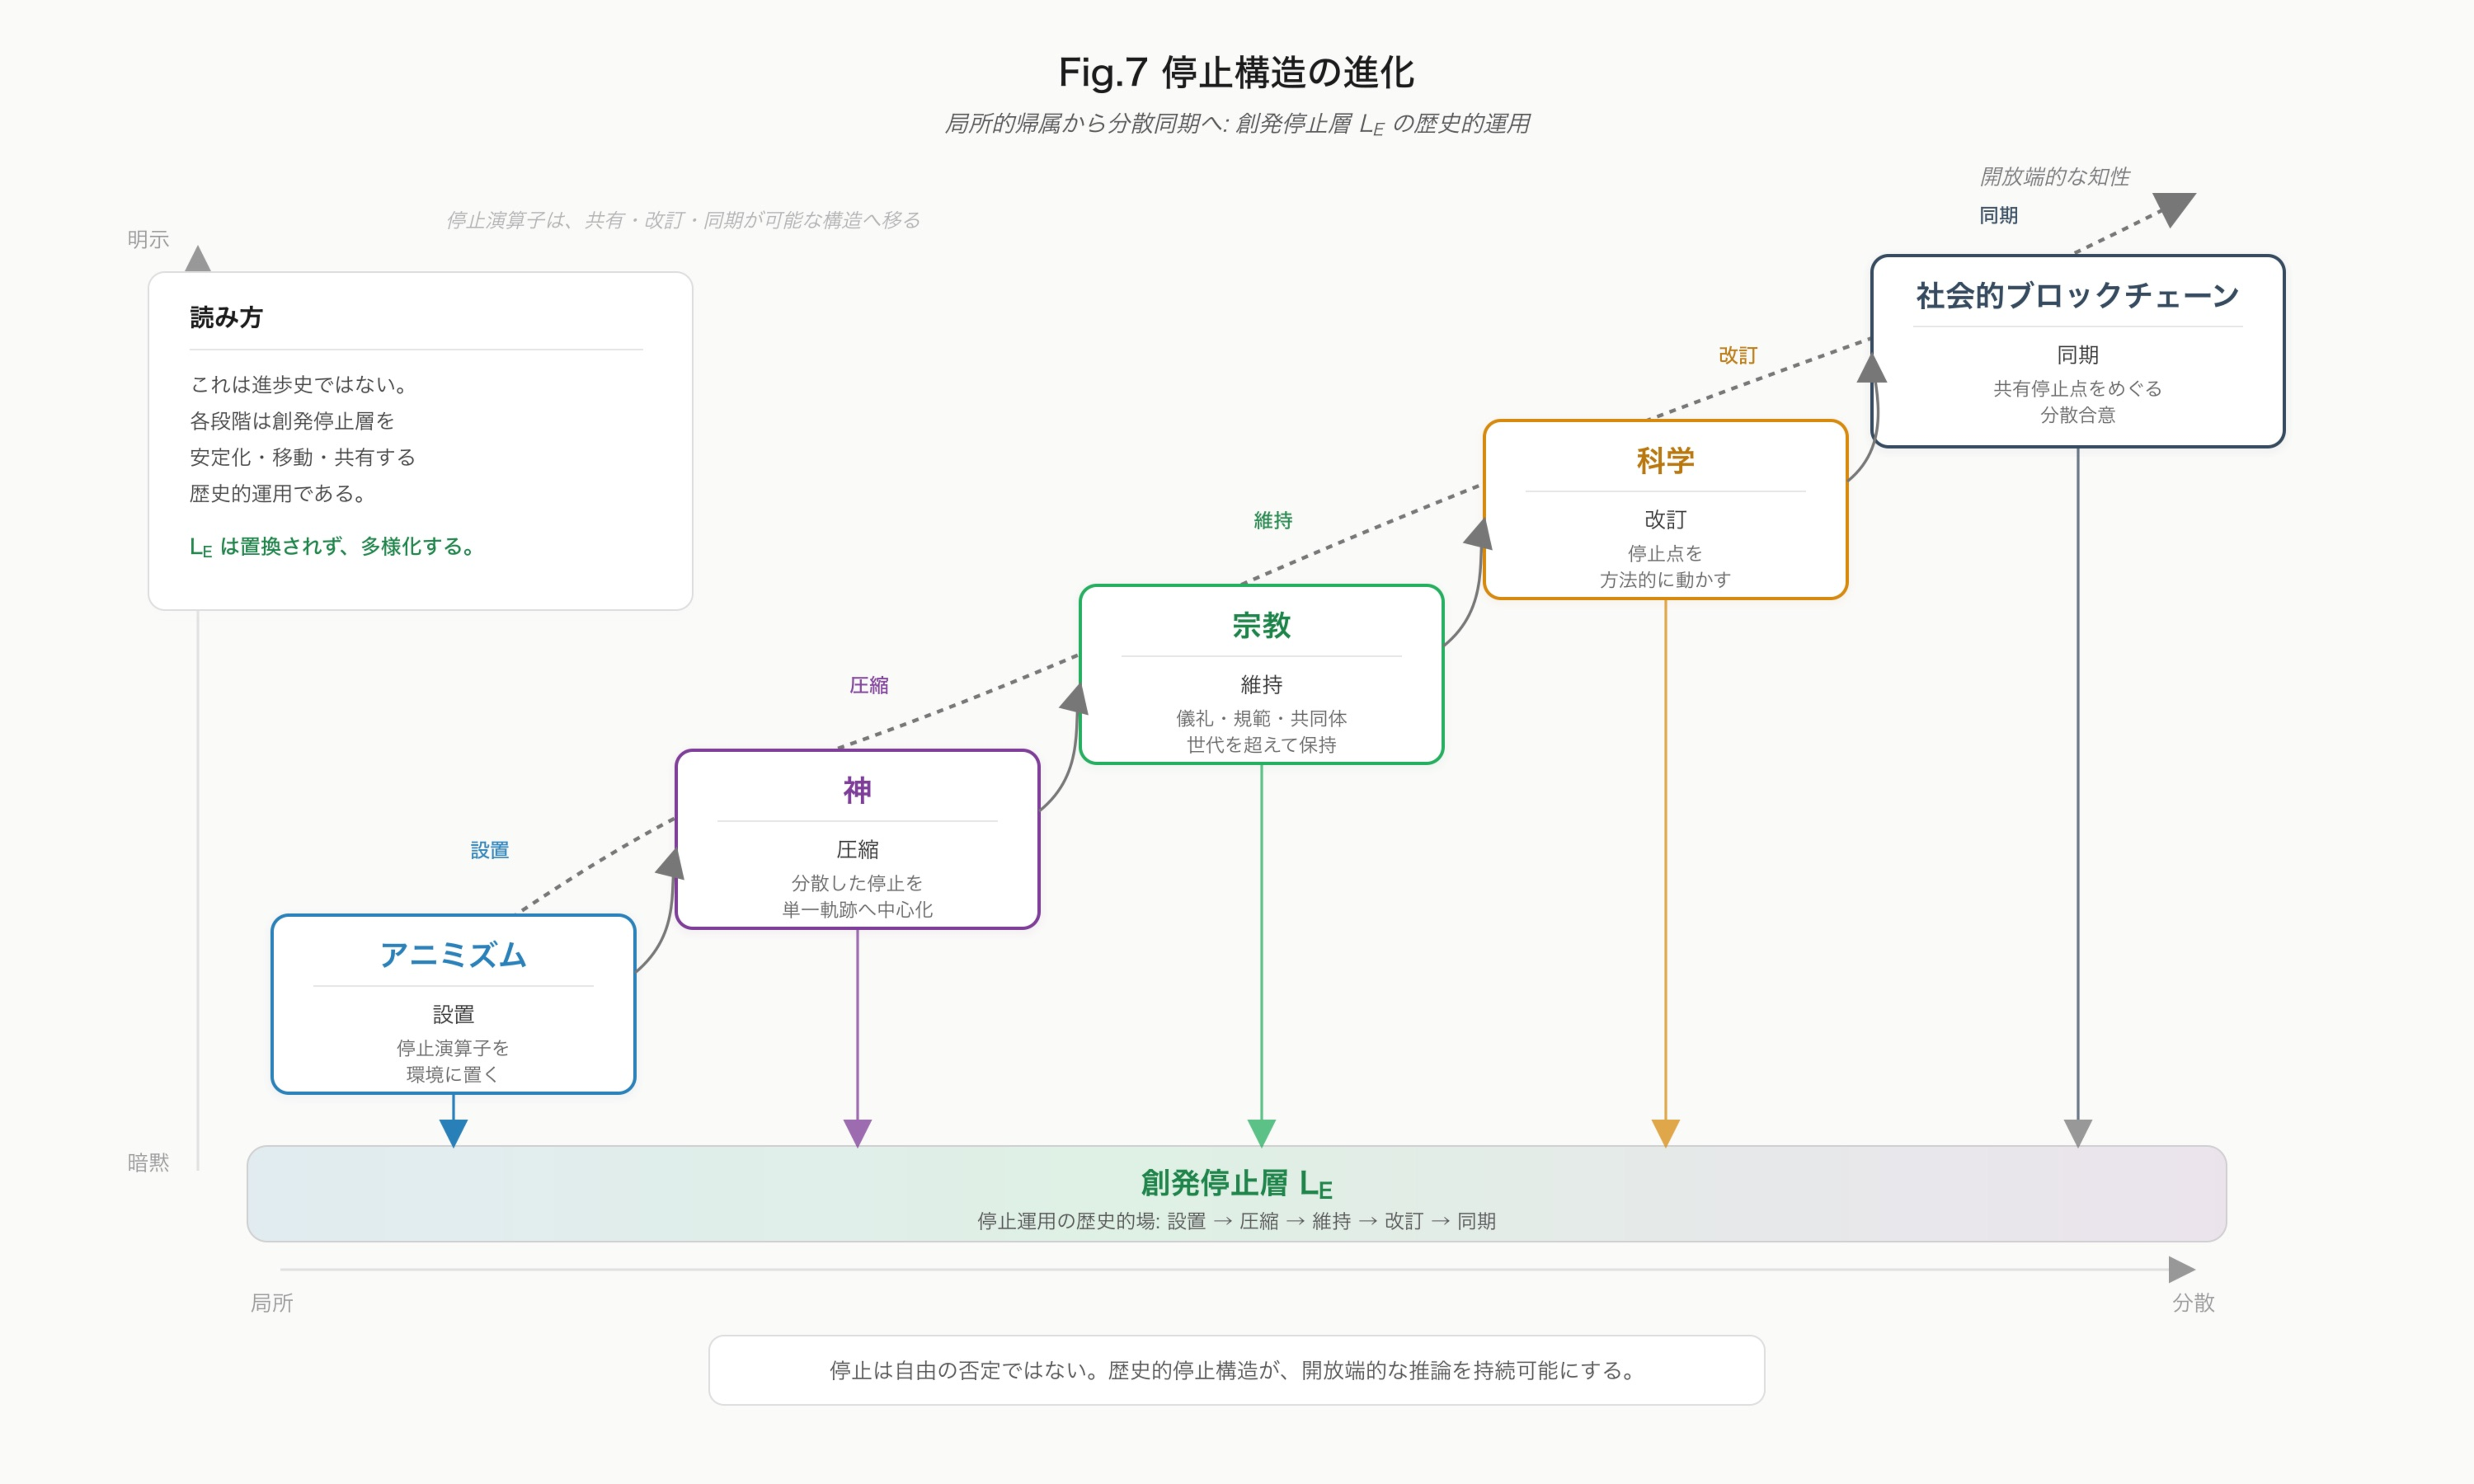
\includegraphics[width=\linewidth]{fig7_evolution_of_stopping_structures_ja.pdf}
\caption{停止構造の歴史的読解の仮説。アニミズム・神・宗教・科学・社会的ブロックチェーンは、モデル内の創発停止層 $L_E$ の役割を安定化・移動・共有するための異なる操作である。}
\label{fig:part2-stopping-evolution}
\figurenote{五つの形態は、設置・圧縮・維持・改訂・同期という停止操作として配置される。これは進歩物語ではなく、$L_E$ の操作レパートリーの多様化である。}{停止は自由の否定ではない。歴史的停止構造は、開かれた推論を有限な系の中で持続可能にするための運用形式として読める。}
\end{figure}

この系列を停止構造の運用史として読めば、さらに位置づけは明確になる。宗教が停止構造の長期維持を制度化した運用形態であるならば、科学は停止構造の更新を制度化した運用形態として理解できる。社会的ブロックチェーンはさらにその上で、停止構造の分散的共有と同期を担う仕組みとして位置づけられる。

重要なのは、これがアニミズムの分散への「回帰」ではないことである(\S{}8.8 で予告)。アニミズムの分散は、個体と環境の直接相互干渉であった。社会的ブロックチェーンの分散は、個体間 $L_E$ の相互干渉ネットワークの運用である。前者は個体−環境の関係、後者は個体−個体の関係である。両者はともに分散的だが、分散している対象が異なる。

本稿はこの構造を、Bio-IFGT がfuture extensionとして開いた個体間共有との提案的類比に置く。ただし、Bio-IFGT に個体間coupling modelや準閉包維持の専用結果はなく、両者のtyped translationも未確立である。社会的ブロックチェーンによる知性の停止構造の議論は本稿側の提案であり、Bioの既成果ではない。

すなわち、個々の $L_E$ は個体内に閉じない。それはノード間相互干渉によって相互に維持される。個体の $L_R$(ログ)が社会的に共有・参照されることで、$L_E$ の分散維持が可能になる。社会的ブロックチェーンは、この分散維持の明示的な構造である。

\bigskip


\subsection{次章への橋渡し}


\S{}6〜\S{}9 では $L_E$ と $\Phi_{\text{net}}$ をアニミズム・神・宗教・社会的ブロックチェーンという役割と比較した。安定性・改訂可能性と停止維持の関係は、各分類の命名から分けた仮説である。

正統性を分散的受容との関係で読む(\S{}9.4)。その受容と停止の関係は仮説であり、真理を保証するものではない。ここから知識の役割を問い、正当化・真理・停止を区別して検討する。

\S{}10 の Gettier 問題は構造的な診断として再解釈する。$C$(閉包度)を真理測度としない定義や、$L_E$ の改訂可能な停止という提案と比較するが、その再解釈を本枠組みの独立証拠にはしない。

\bigskip


\subsection{要約}


本章で示したのは次の点である:

\begin{enumerate}
\item 「社会的ブロックチェーン」は暗号通貨技術ではなく、単一権威なしに停止と更新を両立させる構造のアナロジーである
\item その構成要素は個体ノード・ログ・ブロック・フォーク・マージ/破棄である
\item 技術的バージョン管理と社会的ブロックチェーンの探索/安定化とコストの対比は仮説であり、対称的な反転則ではない
\item 技術的ブロックチェーンは一貫性問題を、社会的ブロックチェーンは正統性問題を扱う。正統性の原理的な非計算可能性は未確立である
\item 正統性と改訂可能性の関係は構造仮説であり、原理的な非計算可能性は確立されない
\item 個体の創造と社会的安定化を役割上対照するが、創造の排他法則ではない
\item 社会的ブロックチェーンは $\Phi_{\text{net}}$ を明示的分散構造として運用する本稿の提案であり、Bio-IFGT のfuture extensionとの関係は未確立の類比である
\item 停止と真理を区別する局所的な読み方を、\S{}10 の Gettier 診断と比較する
\end{enumerate}


次章 \S{}10 では、$C$ が真理測度ではなく安定性測度であることを、ゲティア問題を通じて構造的に診断する。

\bigskip
